\setcounter{page}{1}
\section*{Zielsetzung}
Elektronen in Halbleiternanostrukturen, deren Abmessungen im $\si{\nano\meter}$ Bereich liegen,
erfahren einen räumlichen Einschluss. In kolloidalen Nanokristallen erfolgt dieser Einschluss
in allen drei Raumrichtungen, was zu rein diskreten Energiespektren führt, die von Atomen bekannt sind.
Durch Einstellung der Größe und der chemischen Zusammensetzung lassen sich die opto-elektronischen
Eigenschaften der Kristalle fast beliebig einstellen, was sie aus technischer Sicht extrem interessant macht.
Die räumliche Begrenzung der Elektronen-Wellenfunktionen führt zu einer ausgeprägten Luminszenz, die
in diesem Experiment untersucht werden soll.

\section{Theorie}
Nachfolgend sollen zunächst einige theoretische Überlegungen zu Halbleiter-Nanokristallen vorgstellt werden, die
zum Verständnis der durchgeführten Messungen notwendig sind.

\subsection{Nannokristalle}
Zum Verständnis von Halbleiternanostrukturen ist eine Betrachtung von Banddiagrammen unverzichtbar\footnote{"\textit{If,
in discussing a semiconductor problem, you cannot draw an Energy-Band-Diagram, this shows
that you don't know what you are talking about. If you can draw one, but don't, then your audience
won't know what you are talking about.}"  - H. Krömer}. In solchen Diagrammen sind
die Unterseite des Leitungsbandes und die Oberkante des Valenzbandes einer Heterostruktur gegen eine
räumliche Achse aufgetragen.
\begin{figure}
  \centering
  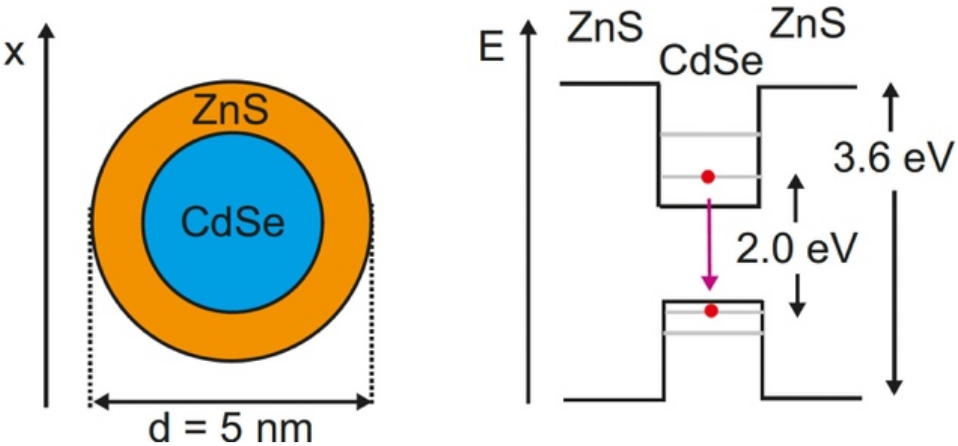
\includegraphics[width = 0.5\textwidth]{pics/banddiagramm.png}
  \caption{Schematische Darstellung eines Nanokristalls aus \ce{CdSe} und \ce{ZnS} (links) und
  das zugehörige Banddiagramm (rechts) \cite{anleitung_pl}.}
  \label{fig: energy_diagram}
\end{figure}
Abbildung~\ref{fig: energy_diagram} zeigt ein solches Diagramm für das hier untersuchte System aus \ce{CdSe} und
\ce{ZnS}. Die räumliche Achse verläuft durch den Mittelpunkt der kugelförmigen Struktur. Aufgrund der Tatsache, dass
die Bandlücke von \ce{CdSe} geringer ist als die von \ce{ZnS}, stellt der Verlauf der Bandkanten sowohl für Elektronen, als auch
für Löcher einen dreidimensionalen Potentialtopf im Inneren der Struktur dar. Das Spektrum der Elektronen bzw. Löcher,
die sich innerhalb des Topfes befinden, lässt sich vereinfacht durch Lösung der Schrödingergleichung berechnen:
\begin{equation}
  \left[-\frac{\hbar^2}{2 m} \Delta^2 + V(\vec{r}) \right] \Psi(\vec{r}) = E \Psi(\vec{r}), \quad
  V(\vec{r}) = \begin{cases}
0,& \quad r > a\\
-V_0,& \quad r \leq a
\end{cases}
\end{equation}
mit der Ausdehnung des Quantentopfes $a$ und dem Einschlusspotential $V_0$.
Im Eindimensionalen Fall lassen sich die Energiezustände
anhand einer Quantenzahl $n \in N$ beschreiben:
\begin{equation}
  E_n = \frac{\pi^2\hbar^2n^2}{ 2 m a^2}.
\end{equation}
Es zeigt sich also, dass die Energien, die letztlich die Lumineszenzenergien festlegen, durch die Größe $a$ der Nanokristalle
moduliert werden können. Diese Eigenschaft bleibt auch im dreidimensionalen Fall erhalten, wobei hier zur Beschreibung der
Energieniveaus $E_{n, l}$ noch eine Drehimpulsquantenzahl $l \in N$ benötigt wird. Da hier stehts mit einem Ensemble von Nanokristallen
in Pulverform gearbeitet wird, ist die Betrachtung von Drehimpulsen jedoch irrelevant.
